\chapter{Einführung}
In Anbetracht der Tatsache, dass neuronale Netzwerke in Zukunft eine grössere Rolle spielen, wird in diesem Dokument
das Ziel verfolgt, die Mathematik dahinter verständlich zu erklären. Es werden einige Vorkenntnisse im Bereich der neuronalen Netze
vorausgesetzt. Dazu gehört das Grundverständnis, wie sich z.B. ein Neuron zusammensetzt, wie sich ein neuronales Netz
zusammensetzt und welche Arten es gibt. In diesem Dokument wird sich lediglich einem Fully-Connected Network gewidmet,
bei welchem die Neuronen nur in eine Richtung verbunden sind. Für Leser, welche sich im Gebiet der
Differentialrechnung und Optimierung noch nicht so gut auskennen, sei hier an dieser Stelle geraten, den Anhang zu lesen.
\\

Grundsätzlich bildet ein neuronales Netz einen gegebenen Input auf einen Output ab, ist also nichts weiteres als
eine Funktion. Diese Funktion wiederum ist mehrdimensional, hat also mehrere Input-Variablen und bildet diese wiederum
auf einen mehrdimensionalen Output ab $f: \mathbb{R}^m \rightarrow \mathbb{R}^n$. Die Input-Variablen sind die Gewichte, die Output-Werte
die Klassen\footnote{Sollen z.B. in einem Bild Hunde und Katzen erkannt werden, so gibt es zwei Klassen \glqq Hund\grqq{} und \glqq Katze\grqq.
In dem Fall ist die Output-Dimension zweidimensional.}. Es werden nun die Gewichte dieses neuronalen Netzes so trainiert, dass eine gewählte Fehlerfunktion
möglichst minimiert wird. Man befindet sich hier im Bereich der Optimierung. In Abbildung \ref{fig:05_approximation}
ist eine solche lineare Funktion (in rot) gegeben, welche die Datenpunkte möglichst optimal annähert.
\begin{figure}[h!]
    \begin{center}
        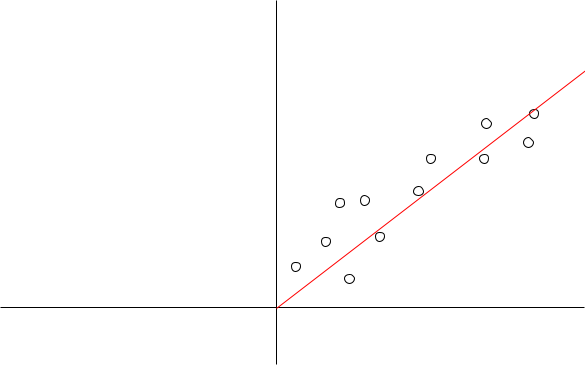
\includegraphics[width=0.3\linewidth]{../common/00_introduction/00_resources/00_approximation.png}
    \end{center}
    \caption{Annäherung an Datenpunkte über lineare Funktion}
    \label{fig:05_approximation}
\end{figure}

Anzumerken sei hier, dass sich der Inhalt des Dokuments auf den Kursteil \glqq Games and Simulations\grqq{} der Vertiefung
\glqq Computer Perception \& Virtual Reality\grqq{} der BFH (Berner Fachhochschule) stützt. Dementsprechend gilt Herrn
Prof. Dr. Jürgen Eckerle ein Dankeschön für die Einführung, welche er an zwei Vorlesungen gegeben hat.